\documentclass[a4paper, 12pt, twoside]{article}
\usepackage[T2A,T1]{fontenc}
\usepackage[utf8]{inputenc}
\usepackage[english, russian]{babel}
\usepackage{graphicx}
\usepackage[hcentering, bindingoffset = 10mm, right = 15 mm, left = 15 mm, top=20mm, bottom = 20 mm]{geometry}
\usepackage{multirow}
\usepackage{lipsum}
\usepackage{amsmath, amstext}
\usepackage{siunitx}
\usepackage{subcaption}
\usepackage{wrapfig}
\usepackage{adjustbox}
\usepackage{enumerate, indentfirst, float}
\usepackage{capt-of, svg}
\usepackage{cmap} % Улучшенный поиск русских слов в полученном pdf-файле

\usepackage{pscyr} % Нормальные шрифты
\usepackage[normalem]{ulem} % для подчёркиваний uline
\ULdepth = 0.16em

\usepackage{fancyhdr} %Колонтикулы
\pagestyle{fancy}
\lhead{
\includegraphics[width = 10 mm]{logo.jpg} Пассивные электрические цепи.}
\rhead{\textit{\today}}

\newenvironment{bottompar}{\par\vspace*{\fill}}{\clearpage}
 
\begin{document}
\begin{titlepage}

\newcommand{\HRule}{\rule{\linewidth}{0.7mm}} % Defines a new command for the horizontal lines, change thickness here

\center % Center everything on the page
 
%----------------------------------------------------------------------------------------
%	HEADING SECTIONS
%----------------------------------------------------------------------------------------

\textsc{\LARGE Московский Физико-Технический Институт}\\[1,5cm] % Name of your university/college

\textsc{\large Лабораторная работа по радиотехническим сигналам и цепям}\\[0.5cm] % Minor heading such as course title

%----------------------------------------------------------------------------------------
%	TITLE SECTION
%----------------------------------------------------------------------------------------

\HRule
\\[0.4cm]
{ \huge \bfseries Пассивные электрические цепи.}
\\[0.4cm] % Title of your document
\HRule
\\[1.5cm]


 
%----------------------------------------------------------------------------------------
%	AUTHOR SECTION
%----------------------------------------------------------------------------------------


	\begin{center} \large
		\textbf{Автор:}\\
		Глеб Уваркин \\
		615 группа
	\end{center}

~


\begin{bottompar}
	\begin{center}
		
\includegraphics[width = 80 mm]{logo.jpg}
	\end{center}
	{\large \today}

\end{bottompar}
\vfill % Fill the rest of the page with whitespace

\end{titlepage}

\section*{Задание №1.Интегрирующие и дифференцирующие звенья.}
'
\subsection*{1.}
	\begin{wrapfigure}[8]{r}{0.2\linewidth}
		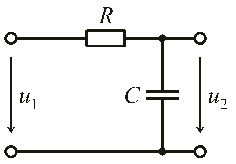
\includegraphics[width =  \linewidth]{integer}
		\caption{Интегрирующая цепь.}
		\label{RLC}
	\end{wrapfigure}	На макетной плате соберём интегрирующую цепь с постоянной времени $\tau \simeq 0.1$ мс, $f_0 = \frac{1}{2\pi \tau} \simeq 1600$ Гц, $R\simeq 100$ Ом, $C \simeq 100$ мкФ.

\subsection*{2.}
Подключим генератор синусоидальных сигналов и осциллограф. Экспериментально оценим верхнюю граничную частоту $f_0$ по уровню $\frac{1}{\sqrt{2}} \simeq 0.7 = -3$dB.

На частоте 10 Гц двойная амплитуда равна $1.946$В.
$1.946 \cdot 0.7 \simeq 1.362$В. На частоте 1.3 кГц получаем двойное напряжение $1.353$В. Значит, \underline{$f_0 \simeq 1.3$кГц.}

Измерим значения коэффициента передачи $K(f) $ на частотах $f=2^n f_0, n = [-2, 4]$.
$$K(f)_{\text{эксп}} = \dfrac{A_{\text{вых}}}{A_{\text{вх}}},$$ где $A_{\text{вх}} = 1$В-амплитуда входного сигнала.
$$ K(f)_{\text{теор}} = \dfrac{1}{\sqrt{1+\left (\dfrac{f}{f_0}\right )^2}} $$

\begin{table}[H]
	\centering
	
	\label{my-label}
	\begin{tabular}{|c|c|c|c|c|c|c|c|}
		\hline
		f, Гц                & 325  & 650  & 1300 & 2600 & 5200 & 10400 & 20800 \\ \hline
		$A_{\text{вых}}$,мв  & 1917 & 1732 & 1345 & 866  & 471  & 247   & 125   \\ \hline
		$K(f)_{\text{эксп}}$ & 0.96 & 0.87 & 0.67 & 0.43 & 0.24 & 0.12  & 0.06  \\ \hline
		$K(f)_{\text{теор}}$ & 0.97 & 0.89 & 0.70  & 0.45 & 0.24 & 0.12  & 0.06  \\ \hline
	\end{tabular}
\end{table}

\begin{figure}[H]
	\centering
	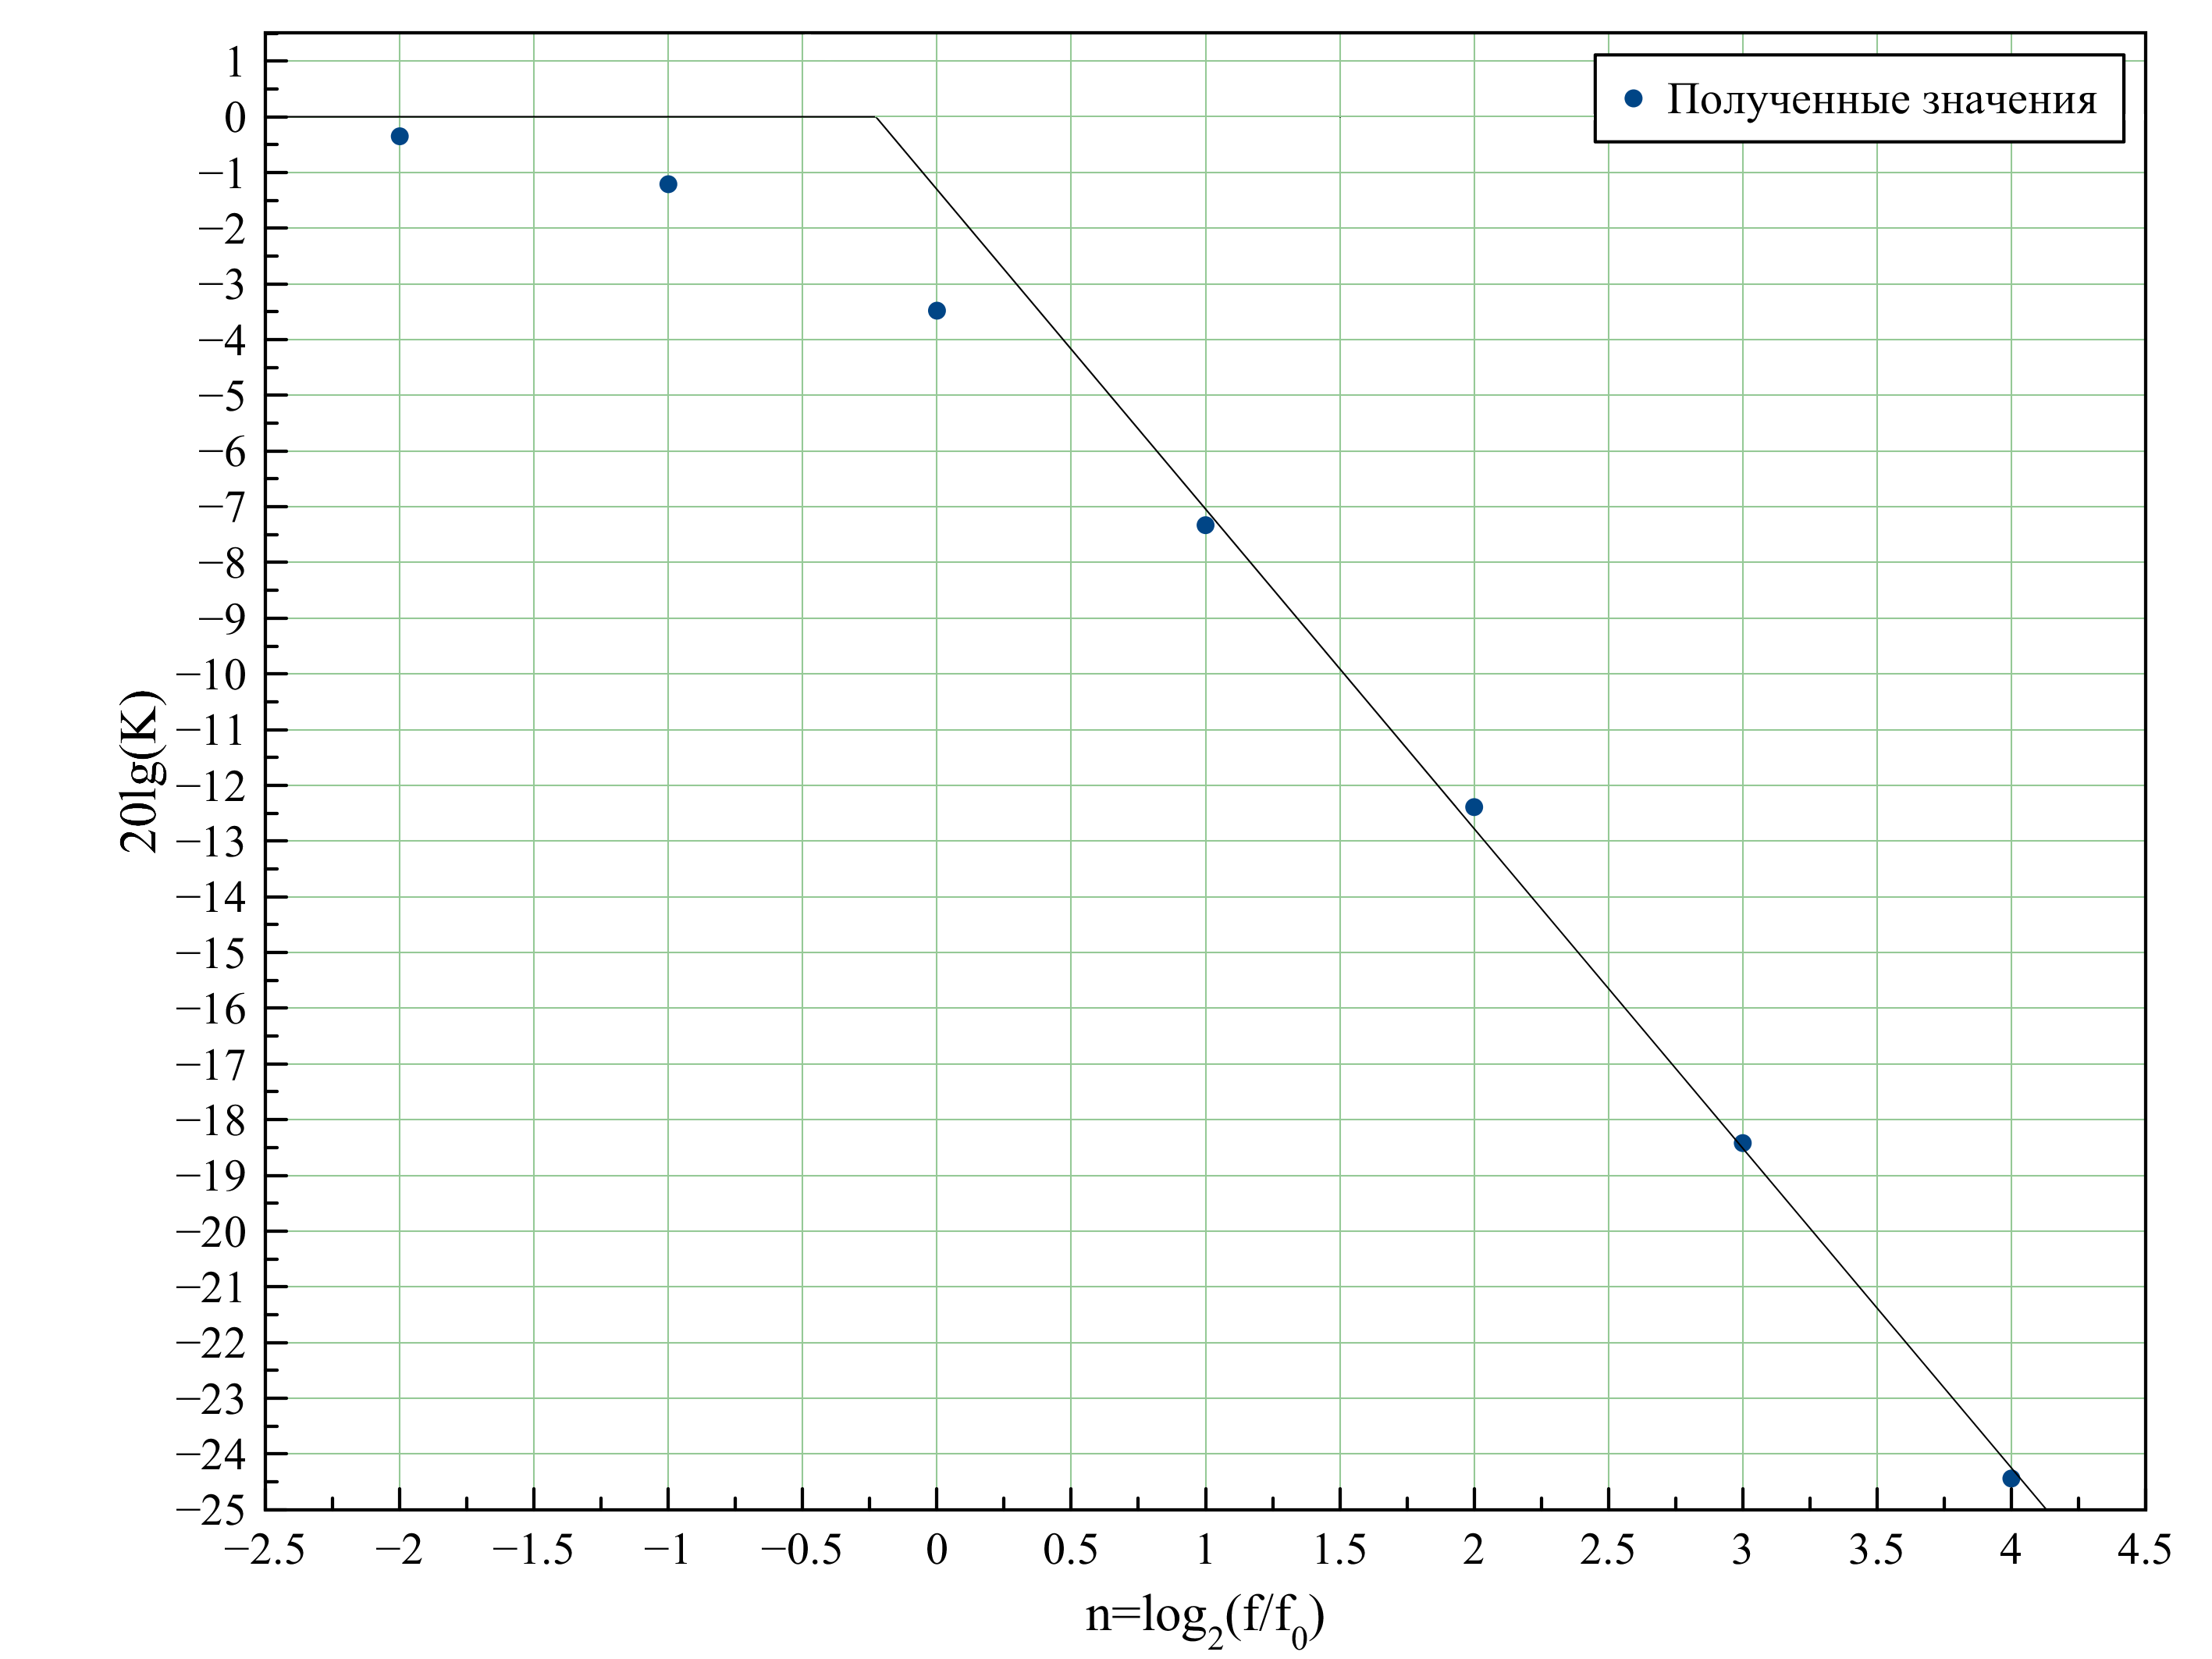
\includegraphics[width = 0.5\textwidth]{bodeint}
	\caption{Граф Боде для интегрирующей цепи.}
\end{figure}

\subsection*{3.}
Подключим генератор прямоугольных сигналов. По осциллограмме переходной характеристики оценим постоянную времени $\tau$, измерив время нарастания фронта импульса от нуля до уровня $1-1/e \simeq 0.63$. Получим \underline{$\tau \simeq 130$мкс}. $f_0 = \frac{1}{2\pi \tau} \simeq 1.2\text{кГц} \simeq 1.3 \text{кГц}$ - рассчитанная частота $f_0$ совпадает с полученной экспериментально, значит равенство $f_0 = \frac{1}{2\pi \tau}$ верно.

\subsection*{4.}
\begin{wrapfigure}[8]{r}{0.2\linewidth}
	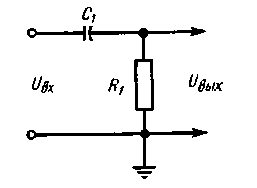
\includegraphics[width =  \linewidth]{diff}
	\caption{Дифференцирующая цепь.}
	\label{RLC}
\end{wrapfigure}
Превратим интегрирующую цепь в дифференцирующую. Оценим нижнюю граничную частоту $f_0$ по уровню $\simeq 0.7 = -3$dB. На частоте 3.03 МГц двойная амплитуда равна 1.309В. $1.309 \cdot0.7\simeq 0.92$В. На частоте 1.3кГц получаем двойную амплитуда $0.95 \simeq 0.92$. Значит, \underline{$f_0\simeq 1.3\text{кГц}$}.

Измерим значения коэффициента передачи $K(f)$ на частотах $f = 2^nf_0, n = [-4,2]$.
$$K(f)_{\text{эксп}} = \dfrac{A_{\text{вых}}}{A_{\text{вх}}}, ~  K(f)_{\text{теор}} = \dfrac{1}{\sqrt{1+\left (\dfrac{f}{f_0}\right )^{-2}}}.  $$

\begin{table}[H]
	\centering
	\begin{tabular}{|c|c|c|c|c|c|c|c|}
		\hline
		f, Гц                & 87.5 & 163  & 325  & 650  & 1300 & 2600 & 5200 \\ \hline
		2$A_{\text{вых}}$,мв & 92.5 & 177  & 346  & 621  & 952  & 1178 & 1280 \\ \hline
		$K(f)_{\text{эксп}}$ & 0.05 & 0.10 & 0.22 & 0.42 & 0.68 & 0.88 & 0.95 \\ \hline
		$K(f)_{\text{теор}}$ & 0.07 & 0.12 & 0.24 & 0.45 & 0.71 & 0.89 & 0.97 \\ \hline
	\end{tabular}
\end{table}

\begin{figure}[H]
	\centering
	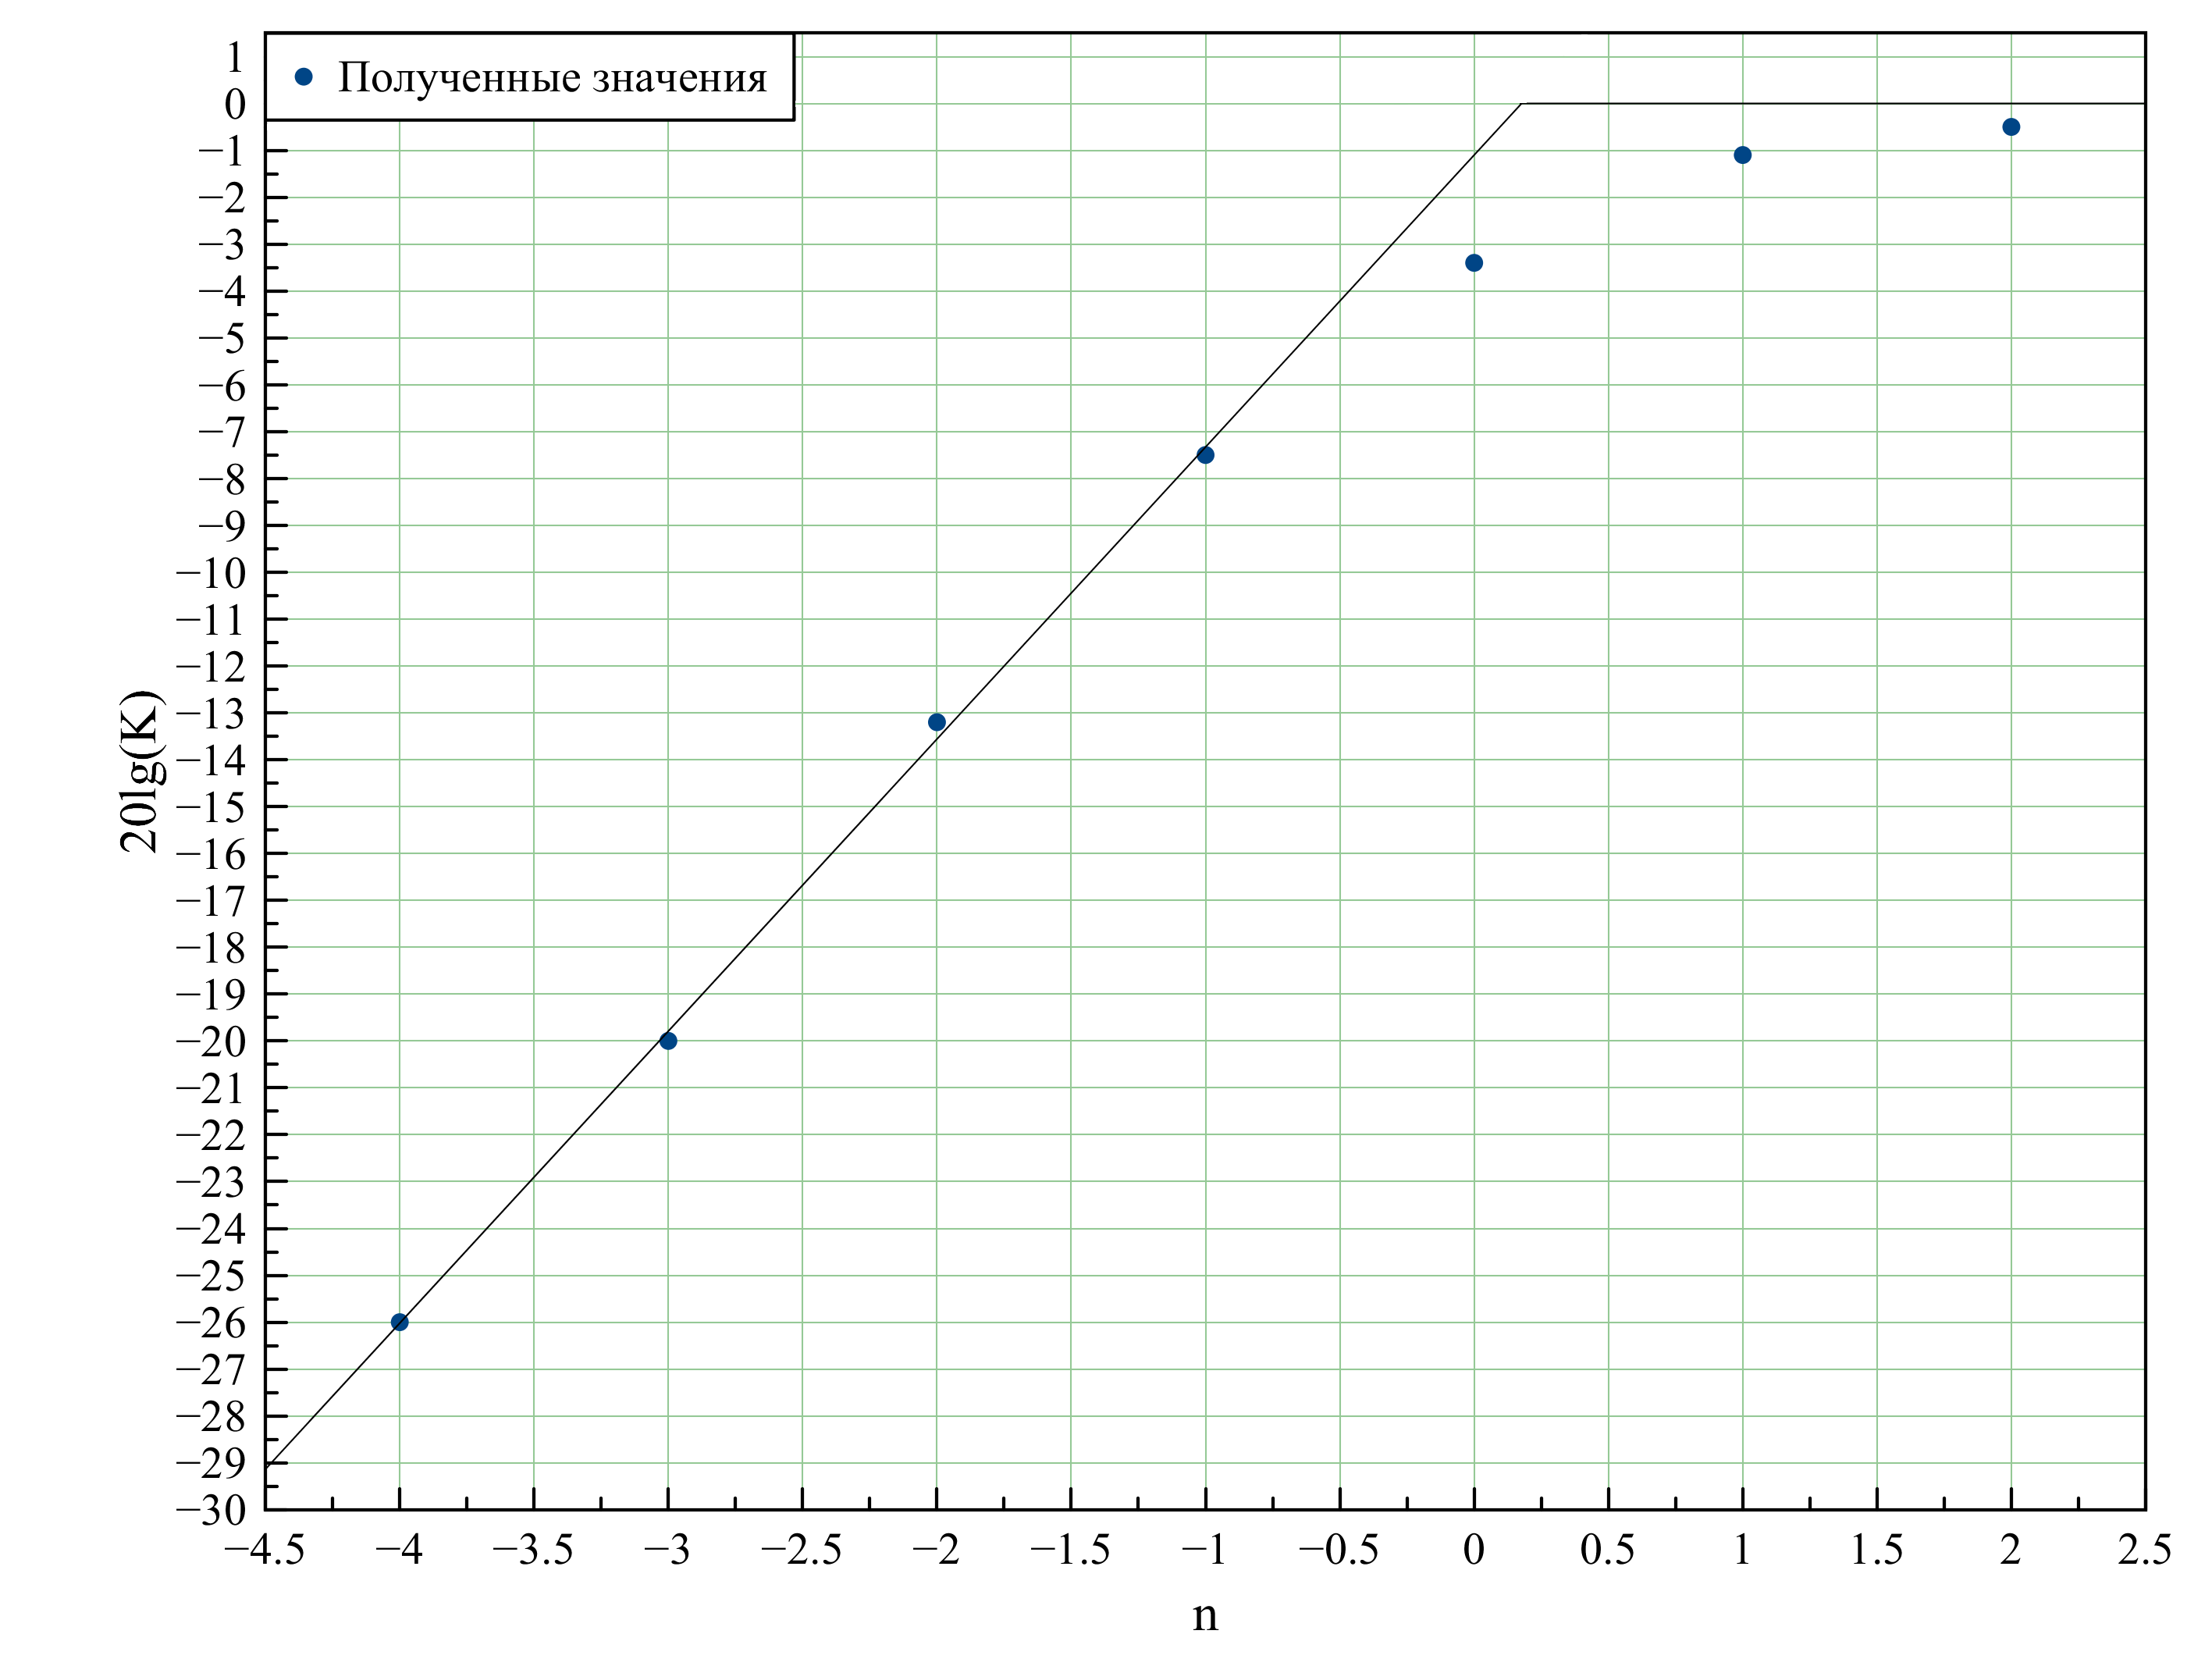
\includegraphics[width = 0.8\textwidth]{bodediff}
	\caption{Граф Боде для дифференцирующей цепи.}
\end{figure}

По осциллограмме переходной характеристики оценим постоянную времени $\tau$, измерив время спада вершины импульса от нуля до уровня $1/e \simeq 0.37$. Получим \underline{$\tau \simeq 125$мкс}. $f_0 = \frac{1}{2\pi \tau} \simeq 1.27\text{кГц}\simeq 1.3{\text{кГц}}$. Теоретическое значение $f_0$ совпадает с экспериментальным - формула $f_0 = \frac{1}{2\pi \tau}$
верна.

\subsection*{5.}

В MicroCap откроем модель \textbf{rcint.cir}.Изучим графики частотной и фазовой характеристик интегрирующей цепи. Оценим ее верхнюю частоту. Получим $f_0 \simeq 10$кГц. Изучим переходную характеристику. По графику оценим постоянную времени. Получим $\tau \simeq 15.903$мкс. Убедимся в том, что при наличии сопротивления $R_L$ передаточная функция цепи принимает вид: $$H(p) = \dfrac{K_0}{1+p\tau},~ K_0 = \dfrac{R_L}{R+R_L},~ \tau =(R||R_L)C.$$

$$K_0 \simeq 1, ~ \tau \simeq 0.1\text{мс}, ~ H(p) = \dfrac{K_0(1-p\tau)}{1-p^2\tau^2} = \dfrac{K_0(1-jw\tau)}{1+w^2\tau^2} = \dfrac{1}{1+\omega^2\cdot10^{-8}} - j\dfrac{\omega \cdot 10^{-4}}{1+\omega^2\cdot10^{-8}}$$

Изобразим график $|H(p)|(\omega)$.

\begin{figure}[H]
	\centering
	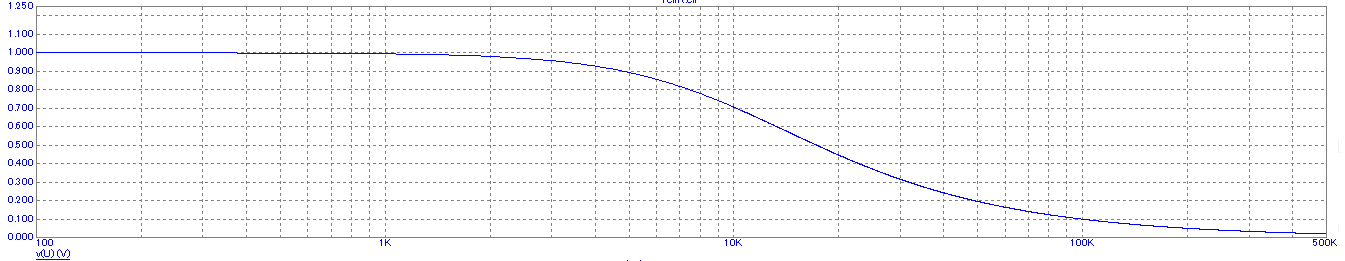
\includegraphics[width = 1\textwidth]{H(p)int}
	
\end{figure}


\subsection*{6.}

Откроем модель \textbf{rcdiff.cir}. Изучим частотную и фазовую характеристики дифференцирующей цепи, оценим ее нижнюю частоту. Получим $f_0 \simeq 10$кГц. Изучим переходную характеристику. По графику оценим постоянную времени. Получим $\tau \simeq 15.9$мкс. Проанализируем влияние резистора $R_S$, задав его варьирование $R_S = [0,10k|10k].$ При увеличении $R_S$ увеличивается время спада вершины импульса, и уменьшается минимальное значение амплитуды.

Убедимся, что при наличии $R_S \neq 0$ передаточная функция принимает вид $$H(p) = \dfrac{K_0 p \tau}{1+p\tau},~ K_0 = \dfrac{R}{R+R_S},~ \tau =(R+R_S)C$$

$$K_0 \simeq 1, ~ \tau \simeq 0.1\text{мс}, ~ H(p) = \dfrac{K_0 p\tau (1-p\tau)}{1-p^2\tau^2} = \dfrac{-K_0 p^2\tau ^2}{1-p^2\tau^2} + \dfrac{K_0 p\tau}{1-p^2\tau^2} = \dfrac{\omega^2\cdot 10^{-8}}{1+\omega^2\cdot 10^{-8}} + j\dfrac{\omega \cdot 10^{-4}}{1+\omega^2\cdot 10^{-8}}$$.

Изобразим график $|H(p)|(\omega)$.

\begin{figure}[H]
	\centering
	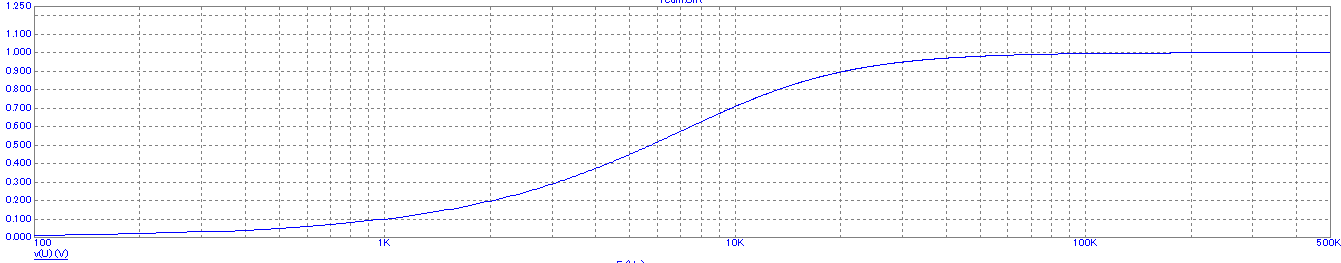
\includegraphics[width = 1\textwidth]{H(p)diff}
	
\end{figure}


\subsection*{7.}


Откроем модель \textbf{rcpower.cir}. Изучим графики частотной зависимости потребляемых интегрирующей цепью активной и реактивной мощностей и графики мощностей на ее компонентах. 

Проверим выполнение закона сложения мощностей на граничной частоте $f_0 = 10$к. Закон сложения мощностей выполняется, так как активная мощность, потребляемая цепью, равна мощности активного сопротивления $R: W \simeq 0.5$мВт, а реактивная - конденсатора $C:W\simeq -0.5$мВт. Подключая и отключая резистор $R_L$ варьированием $[1k,1Meg|1Meg]$. Изучим его влияние на распределение  мощностей в схеме при $f=f_0$. При уменьшении $R_L$ до 1k при $f_0$ его полная мощность возрастает до 0.2 мВт, мощность на R падает до 0.4 мВт, а реактивная мощность конденсатора становится равной -0.2 мВт.
\begin{figure}[H]
	\centering
	\begin{minipage}[h]{0.47\linewidth}
		\centering{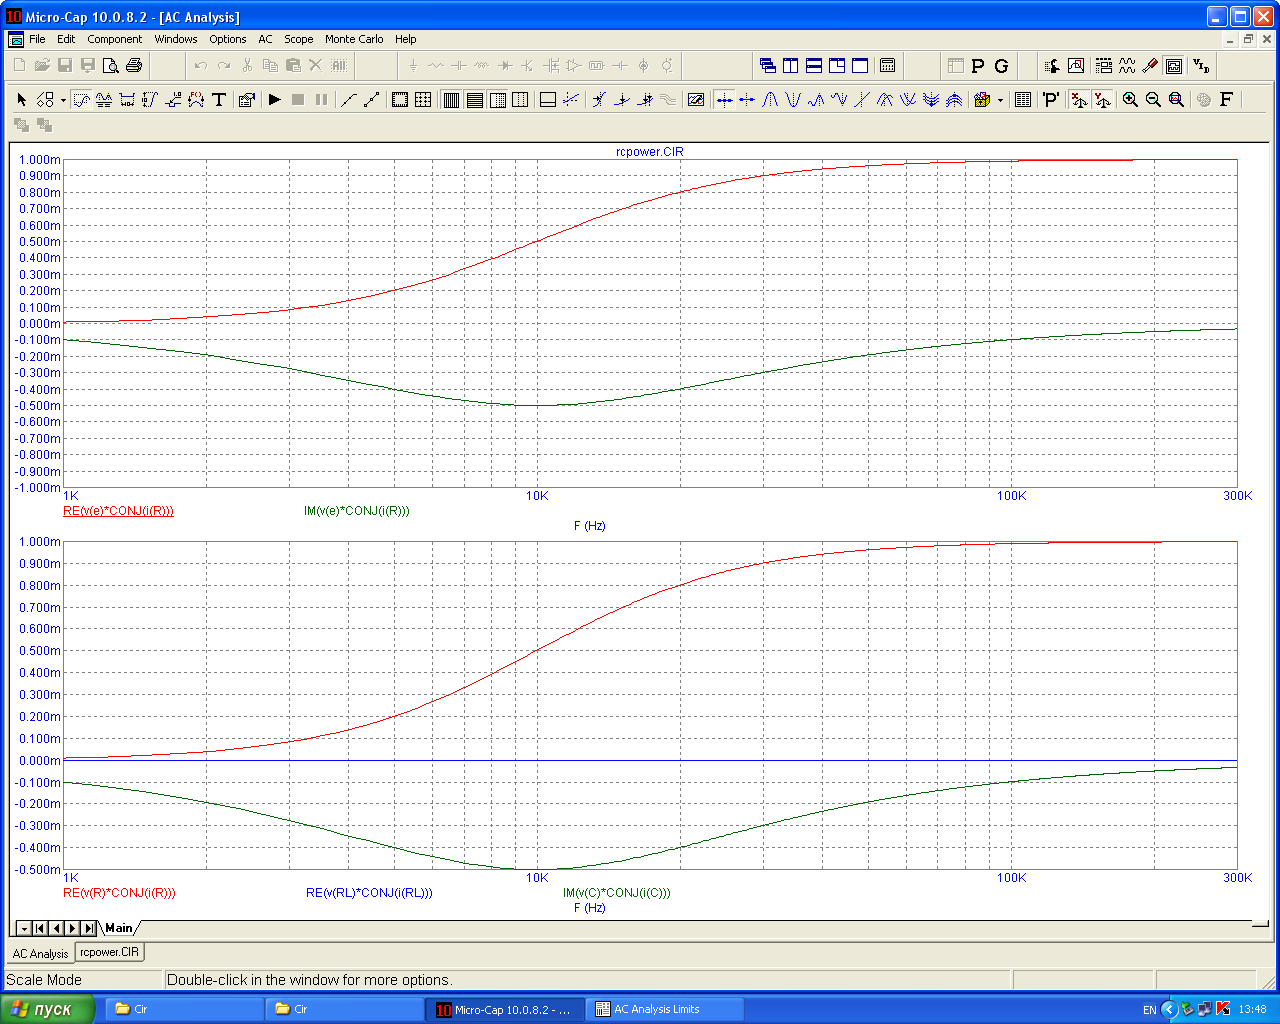
\includegraphics[width=0.9\linewidth]{rcpower.png}\\а) режим AC. }
	\end{minipage}
~
	\begin{minipage}[h]{0.47\linewidth}
		\centering{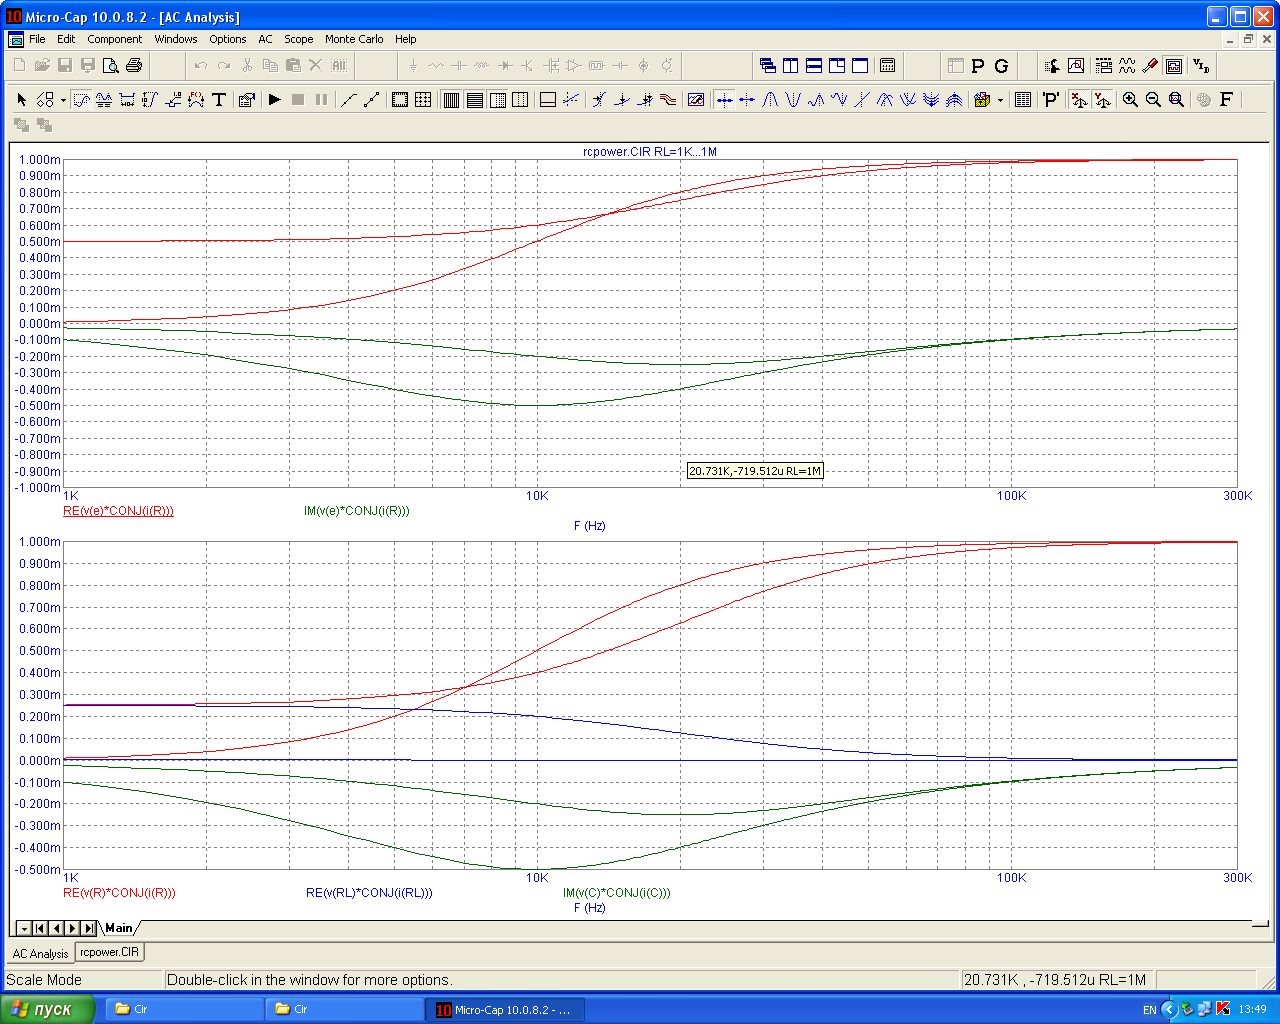
\includegraphics[width=0.9\linewidth]{rcpower-stepping}\\ б) Варьирование $R_L$.}
	\end{minipage}
\end{figure}
\newpage

\section*{Задание 2.RC-звенья второго порядка.} 

\begin{figure}[H]
	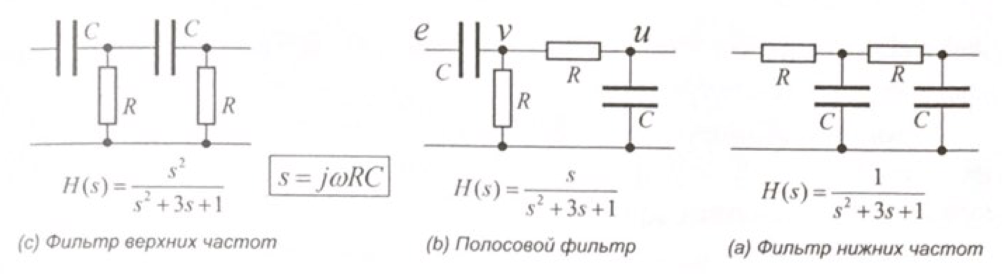
\includegraphics[width =  0.9\linewidth]{RC}
	\caption{Три варианта звеньев второго порядка.}
	
\end{figure}
\subsection*{1.}


Откроем модель \textbf{rc2pole.cir}. По графикам АЧХ и ФЧХ определим затухание на частоте $f_0=\frac{1}{2\pi RC}=9.948$ кГц, которое составила 9.51 dB и скорость его нарастания в полосах задержания -40.69+9.5=-31.18 dB/декаду. По графикам ФЧХ измерим значения фазовых сдвигов ФВЧ, ПФ и ФНЧ на частотах 0, $f_0$, $\infty$. 

\begin{table}[H] 
	\centering 
	\caption{Значения фазовых сдвигов} 
	\label{table2.1} 
	\begin{tabular}{|c|c|c|c|} \hline
		& ФВЧ & ПФ & ФНЧ  \\ \hline
		0 & 180 & 90 & 0  \\  \hline
		$f_0$ & 90 & 0 & -90 \\ \hline
		$\infty$ & 0 & -90 & -180 \\ \hline
	\end{tabular} 
\end{table} 
Двухсторонняя полоса $\Delta f$ пропускания ПФ = 30 кГц, что в три раза больше $f_0$. Это сходится с теорией. 
\subsection*{2.} 
 
Открыв графики переходных характеристик, оценим время спада $\tau_{-}$ первого выброса переходной характеристики ФВЧ до уровня $e^{-1}$ и время $\tau_{+}$ нарастания фронта переходной характеристики ФНЧ до уровня $1-e^{-1}$. $$\tau_{+}=47.33\text{ мс},\;\tau_{-}=3.67\text{ мс}\rightarrow\frac{\tau_{+}}{\tau_{-}}=12.89$$

\newpage

\section*{Задание №3.Мостовые схемы.}

\begin{figure}[H]
	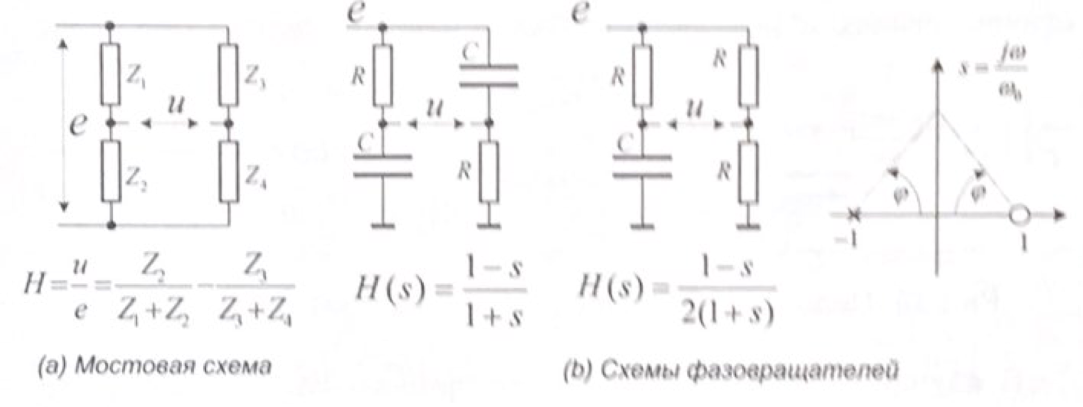
\includegraphics[width =  0.8\linewidth]{most}
	\caption{Мостовые схемы.}
	\label{RLC}
\end{figure}

\subsection*{1.} 
Откроем модель фазовращателя. На частоте $f=25$ кГц реализуется наибольший диапазон перестройки фазы при варьировании $R=[1k,15k|2k]$, границы этого диапазона $\varphi=[-150,73^\circ;-28.54^\circ]$. 

\subsection*{2.} 
Откроем модель двойного Т--моста. Изучим его частотную и фазовую характеристики. Измерим ширину полосы режекции $\Delta f=41.75k-2.37k=39.38k\simeq4f_0$. Изучим поведение характеристик при варьировании $R=[3k,7k|1k]$ и $[4.8,5.2k|0.1k]$. При росте $R$ $f_0$ падает, при $R=5k$ наблюдается скачок на ФЧХ. 

\subsection*{3.} 
Подключим ко входу источник прямоугольного импульса и проанализируем переходную характеристику. Оценим время спада $\tau_{-}=3.9$ мкс и нарастание $\tau_{+}=59$ мкс, что совпадает с теорией $\tau_{+}=\frac{1}{2\pi f_0 \mu_{\pm}},\mu_{\pm}=2\pm\sqrt{3}$. Варьирование $R=[3k,7k|2k]$ приводит к усреднению функции. 

\subsection*{4.} 
Оценим частоты $f_0$ и добротность $Q=\frac{f_0}{\Delta f}$ нулей передачи при $R=[4.9k,5.1k|0.3k]$ 

\begin{table}[H] 
	\centering 
	\label{table3.1} 
	\begin{tabular}{|c|c|c|c|} \hline 
		$R,$ кОм & 4.9 & 5 & 5.1 \\ \hline 
		$f_0$, кГц & 10.05 & 10 & 9.95 \\ \hline 
		$\Delta f$, кГц & 0.1 & 0.001 & 0.1 \\ \hline 
		$Q$ & 100.5 & 1000 & 99.5 \\ \hline 
	\end{tabular} 
\end{table} 
Подключим источник $E_1$ двухчастотного сигнала $\sin 2\pi(f-df)t+\sin 2\pi(f+df)t,\;df=25$. Измерим $\tau_g$: 
$$R=4.9k,\quad f=10.05k\Rightarrow\tau_g=3\text{ мс};\quad\quad\tau_{g\text{ теор.}}=\frac{Q}{\pi f}=3.18\text{ мс}$$ 
$$R=5.1k,\quad=9.95k\Rightarrow\tau_g=3\text{ мс};\quad\quad\tau_{g\text{ теор.}}==\frac{Q}{\pi f}=3.18\text{ мс}$$

\section*{Задание №4.Последовательный резонанс.}

\begin{figure}[H]
	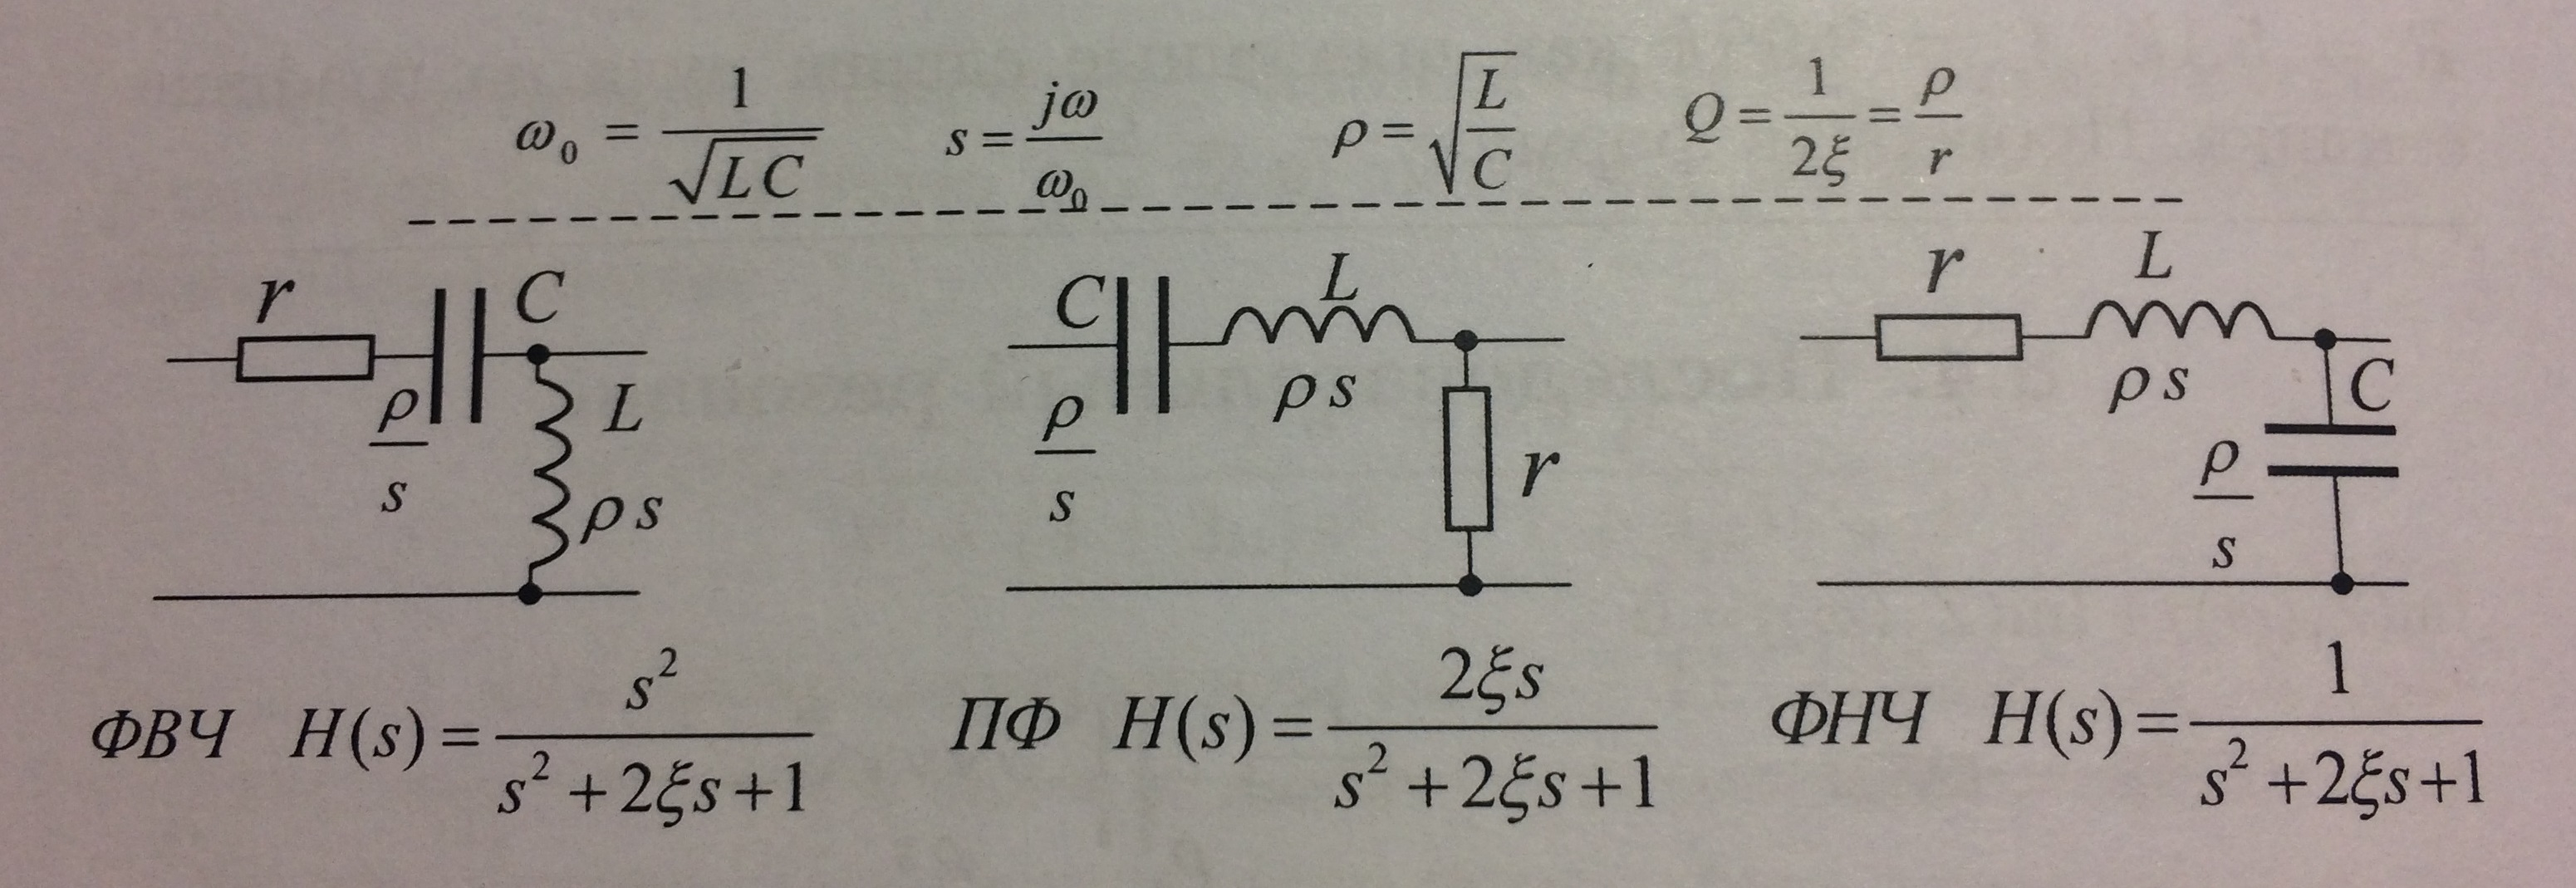
\includegraphics[width =  0.9\linewidth]{poslrez}
	\caption{Двухполюсные резонансы.}
	
\end{figure}
\subsection*{1.}
На макетной плате соберём схему полосового фильтра, выбрав $L\sim 200\mu, ~ C\sim 1000p,~r\sim 90 (f_0 \sim 360k,~\rho ~ 450, Q\sim 5)$. Подключив генератор синусоидального сигнала, измерим резонансную частоту $f_0 \simeq 364k$ , коэффициент передачи $K(f_0) \simeq 1.103$ и ширину $\Delta f$ пика по уровню $0.7 = -3dB$ : $\Delta f = 431-307 = 124k$. Оценим добротность как $Q = f_0/\Delta f = 364/124 \simeq 2.94$.

\subsection*{2.}
Из тех же компонент соберём схемы фильтров верхних (ФВЧ) и нижних (ФНЧ) частот. Измерим отношения $K(f_0)/K(0) \simeq 5.778/1.769 \simeq 3.27$ для ФНЧ и $K(f_0)/K(\infty)\simeq 5.91/1.618 \simeq 3.65$ для ФВЧ.

\subsection*{3.}
Подключив генератор прямоугольных импульсов, изучим переходные характеристики ФВЧ, ПФ, и ФНЧ. Прикинув по осциллограммам период колебаний и время их затухания до уровня $1/e = 0.37$, дадим оценку резонансной частоты $f_0$ и добротности $Q$.

\begin{table}[H] 
	\centering 
	
	\begin{tabular}{|c|c|c|c|c|} \hline
		
		Вид схемы & $T$, мкс & $\tau,$ мкс & $f_0,$ кГц & Q \\ \hline
		ФВЧ & 2.40 & 2.84 & 366 & 7.1 \\ \hline
		ФНЧ & 3.29 & 2.62 & 392 & 4.9 \\ \hline
		ПФ & 2.81 & 2.83 & 366 & 6.1 \\\hline 
	\end{tabular} 
\end{table} 
$$\xi=\frac{1}{\omega_0T}=\frac{2\pi}{f_0T};\; \sqrt{1-\xi^2}=\frac{2\pi}{\omega_0\tau}\Rightarrow1-\frac{1}{\omega_0^2T^2}=\frac{4\pi^2}{\omega_0^2\tau^2}$$ 
$$\omega_0=\sqrt{\frac{4\pi^2}{\tau^2}+\frac{1}{T^2}}\Rightarrow f_0=\sqrt{\frac{1}{\tau^2}+\frac{1}{4\pi^2T^2}}$$

\subsection*{4.}
Откроем в MicroCap модель \textbf{rlc2pole.cir}, изучим частотные фазовые и переходные характеристики фильтров. Сравним результаты моделирования с экспериментом.

\subsection*{5.}

Откроем модель \textbf{groupdel.cir} полосового фильтра с $f_0 = 100k, ~ \rho = 2k$. Наблюдая в режиме Transient отклик на двухчастотный сигнал $\sin 2\pi (f-df)t + \sin 2\pi(f + df)t$, изучим зависимость групповой задержки $\tau_{g}$ от $R = 10,20,40,100.$. Сравним результаты с теорией: $\tau_{g} = -\dfrac{d\phi}{d\omega} = \dfrac{Q}{\pi f_0}$.

\begin{table}[H]
	\centering
	
	
	\begin{tabular}{|c|c|c|c|c|}
		\hline
		R, Ом                    & 10   & 20   & 40   & 100  \\ \hline
		$\tau_g$, мс             & 0.65 & 0.30 & 0.15 & 0.06 \\ \hline
		$\tau_{\text{теор}}$, мс & 0.64 & 0.32 & 0.16 & 0.06 \\ \hline
		Q                        & 200  & 100  & 50   & 20   \\ \hline
	\end{tabular}
\end{table}

\subsection*{6.}

Откроем модель \textbf{lcpower.cir}, изучим графики распределения мощностей в резонансной LRC-цепи. Проверим выполнение закона суммирования мощностей на частоте резонанса и на границах полосы пропускания:

На частоте резонанса($f_0 = 250k$).

$P_L = 177.143m, ~ P_C = -178.571m,~P_R = 18.571m\Rightarrow \sum P \simeq 17.14m$.

На границах полосы пропускания: $f_1 = 238k, f_2 = 262k.$

$f_1$: $P_L = 85.06m,~P_C=-87.83m,~ P_R = 9.36m \Rightarrow \sum P \simeq 6.59m$

$f_2$: $P_L = 88.71m, ~ P_C = -89.54m, ~ P_R = 8.75m \Rightarrow \sum P \simeq 7.92m$.

Закон суммирования выполняется.

\newpage



\section*{Задание №5.Параллельный перенос.}

\begin{figure}[H]
	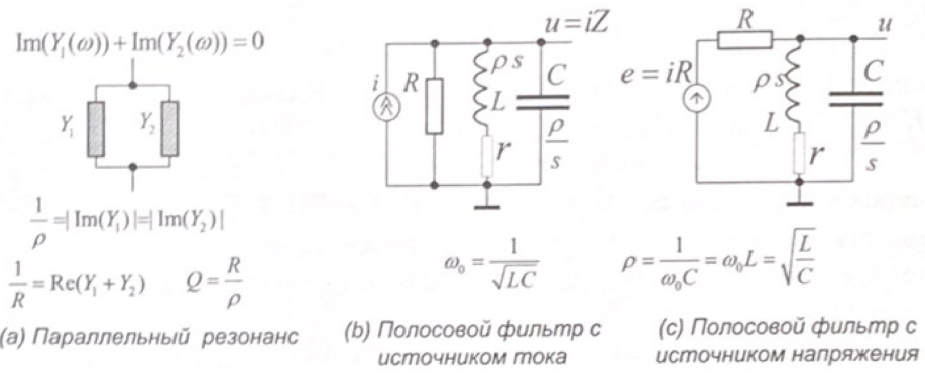
\includegraphics[width =  0.9\linewidth]{parrez}
	\caption{Явление параллельного резонанса.}

\end{figure}

\subsection*{1.}
Откроем в MicroCap модель \textbf{parallel.cir} параллельного контура с $f_0 = 100k, \varrho = 570$. По схеме оценим параметры $\alpha = \frac{\rho}{R_0}, ~\beta = \frac{R}{\rho}, ~ Q = \frac{1}{\alpha + \beta},$ где $\rho = \sqrt{\frac{L}{C}} = \sqrt{\dfrac{905\cdot10^{-6}}{2800\cdot10^{-12}}} \simeq 569 $ Ом. Получаем \underline{$\alpha = \dfrac{569}{10000} \simeq 0.057,~ \beta = \frac{32}{569} \simeq 0.056, ~ Q = \frac{1}{0.057+0.056} \simeq 8.85$}.

\subsection*{2.}

Измерим сопротивление контура $R_0$ на резонансной частоте и полосу $\Delta f$ пропускания по уровню $0.7 = -3$dB. Получаем $R_0 \simeq 5 $ кОм, $\Delta f \simeq 11.15$ кГц. Оценим его добротность как $Q = \frac{R_0}{\rho} = \frac{5000}{569} \simeq 8.79$ и $Q = \frac{f_0}{\Delta f} = \frac{100000}{11150} \simeq 0.89$

\subsection*{3.}

Изучим влияние на добротность последовательных потерь $R$, установив варьирование $R = [0,32|32]$.Измерим добротность при R = 0: $Q =\frac{100000}{5775} \simeq 17.3$. 

Изучим влияние параллельных потерь $R_0$, установив варьирование $R_0 = [10k,1000k|1000k]$. Измерим добротность при $R_0 = 1000$ кОм: $Q = \frac{100000}{5658} \simeq 17.7$. Оценим вклады каждого из резисторов $R, R_0$ в затухание $\frac{1}{Q}$.  При увеличении $R$ от 0 Ом до 32 Ом, затухание меняется с $0.057$ на $0.116$. При увеличении $R_0$ от 10 кОм до 1000 кОм  затухание меняется с $0.114$ на $0.056$.

\subsection*{4.}

Изучим зависимость частоты параллельного резонанса от $R = [0,150|50]$. Частоту резонанса измерим по пересечению нуля фазовой характеристикой. Проверим формулу $f = f_0\sqrt{1-\beta^2}$.

\begin{table}[H]
	\centering
	\caption{Подтверждение формулы $f = f_0\sqrt{1-\beta^2}$.}
	
	\begin{tabular}{|c|c|c|c|c|}
		\hline
		R, Ом             & 0   & 50   & 100  & 150  \\ \hline
		$f_{\text{эксп}}$ & 100.0 & 99.6 & 98.4 & 96.5 \\ \hline
		$\beta$           & 0.00   & 0.14 & 0.18 & 0.26 \\ \hline
		$f_{\text{теор}}$ & 100.0 & 99.0   & 98.4 & 96.6 \\ \hline
	\end{tabular}
\end{table} 

\subsection*{5.}

Исследуем влияние последовательности потерь в области низких частот. Для этого установим частотный диапазон от 1k до 130k и будем варьировать $R = [0,20|2]$. Получим, что при сопротивлении $R = 12$ Ом фазовый сдвиг на частоте 2k составляет $\pi/4$. 

\newpage

\section*{Задание №6.Смешанные резонансы.}

\begin{figure}[H]
	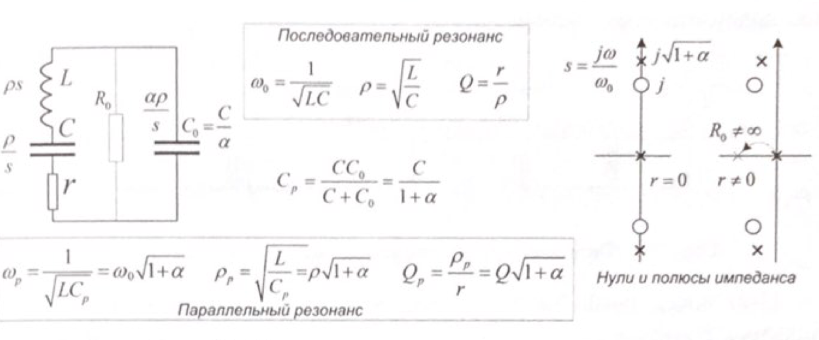
\includegraphics[width =  0.9\linewidth]{smrez}
	\caption{Контур со смешанным резонансом.}
	\label{RLC}
\end{figure}

\subsection*{1.}
Откроем модель \textbf{combined.cir} с $f_0 = 100k,~\rho = 15.9k,~Q\simeq 10,~\alpha = 1$. Изучим графики частотной и фазовой характеристик, а также графики частотных зависимостей вещественной и мнимой частей импеданса.
\subsection*{2.}
Измерим частоты $f_p,f_0$ последовательного и параллельного резонансов по точкам пересечения нуля фазовой характеристикой. Имеем $f_0 \simeq 100.5k,~f_p\simeq 140.6k$. Измерим полюсы $\Delta f_p, \Delta f_0$, в которых фазовая характеристика изменяется в диапазоне $\pm 45$ в окрестностях резонансов. Имеем $\Delta f_p \simeq = 10.7k, \Delta f_0 = 10.4k$.  Рассчитаем добротность $Q_p=\frac{f_p}{\Delta f_p} = \frac{140.6k}{10.7k} \simeq 13.1,~ Q = \frac{f_0}{\Delta f_0} = \frac{100.5k}{10.4k} \simeq 9.66$. Проверим, что $f_p = f_0\sqrt{2}$: $140.6k \simeq 141.4k$ и $Q_p = Q_0\sqrt{2}$: $13.1 \simeq 13.7$.

\subsection*{3.}
Измерим сопротивление контура на частотах последовательного и параллельного резонансов, сравним результаты с теоретическими значениями: $r, k^2\rho_p Q_p$. 

$r_{\text{эксп}} = 1.57k\simeq 1.59k = r_{\text{теор}}$

$(k^2\rho_p Q_p)_{\text{эксп}} = 78k \simeq 79k = \left (\dfrac{\alpha}{1+\alpha}\right )^2\sqrt{\dfrac{L}{C}}(1+\alpha)\dfrac{r}{\rho}  = \left(k^2\rho_p Q_p\right)_{\text{теор}}$

Снимем зависимости сопротивления на частоте параллельного резонанса от $R = [500:2000|500]$ и ёмкости $C_0 = [100p,300p|100p]$. Сопоставим их с теорией. Осмыслим характер изменения графиков при варьировании $R$ и $C_0$.

\begin{table}[H]
	\centering
	\caption{Варьирование $R$.}
	
	\begin{tabular}{|c|c|c|c|c|}
		\hline
		R, Ом  & 500 & 1000 & 1500 & 2000 \\ \hline
		Z, кОм & 220 & 121  & 82   & 63   \\ \hline
	\end{tabular}
\end{table}

$Z \sim \dfrac{1}{R}$

\begin{table}[H]
	\centering
	\caption{Варьирование $C_0$.}
	
	\begin{tabular}{|c|c|c|c|}
		\hline
		$C_0,$ пФ & 100 & 200 & 300 \\ \hline
		Z, кОм    & 68.6 &26.3   & 14.3  \\ \hline
	\end{tabular}
\end{table}

$Z \sim \dfrac{1}{C_0^2}$.

\subsection*{4.}

Обнулим последовательности потери $r$ и варьированием $R_0 = [10k, 100k|10k]$ подберём сопротивление параллельных потерь так , чтобы достичь того же резонансного сопротивления что и при $r = 1590$. Получим $R_0 = 80k$. Проверим закон пересчёта: $R_0 r = k^2 \rho_{p}^2$. $80000\cdot 1590 \simeq \left(\frac{1}{2}\right)^2\cdot (15900)^2\cdot 2$ - соотношение выполняется.

\subsection*{5.}
Варьируя $R_0 = [80k,10Meg|10Meg]$ при $r = 1590$, изучим влияние $R_0$ на поведение частотной и фазовой характеристик на низких частотах - в диапазоне 1k, 180k.
При увеличении $R_0$ частотная характеристика увеличивается, а фазовая уменьшается.




\end{document}
